\addcontentsline{toc}{part}{Day 3: Advanced Kuali Identity Managemet}
\part*{Day 3\\
Advanced Kuali Identity Management}

\addcontentsline{toc}{section}{Exercise4: ldapsearch Tool and Query Syntax}
{\setlength{\baselineskip}%
  {0.0\baselineskip}
  \section*{\flushright Exercise 4\\
ldapsearch Tool and the Query Syntax}
  \hrulefill \par}

\addcontentsline{toc}{subsection}{Description}
\subsection*{Description}
Use the ldapsearch tool to try various query examples in order to find
specific users with different information.

\addcontentsline{toc}{subsection}{Goals}
\subsection*{Goals}
\begin{itemize}
  \item Learn LDAP Query Syntax
  \item Learn to use OpenLdap tools
\end{itemize}

\addcontentsline{toc}{subsection}{Instructions}
\subsection*{Instructions}
\begin{enumerate}
\item Start by verifying the tools are installed by running ldapsearch
  on the commandline by with '-h' to access the help information
\begin{lstlisting}[language=bash,basicstyle=\scriptsize,backgroundcolor=\color{ubergray},caption={Verify
  the ldapsearch is there},frame=single,breaklines=true]
ldapsearch -h
man ldapsearch
\end{lstlisting}
\item Search by connecting to the localhost LDAP server to the
  \textbf{cn-admin,dc=rsmart,dc=com} distinguished name and the
  \textbf{ou=people,dc=rsmart,dc=com} organizational unit, and query
  for anyone with the \textbf{eduPersonPrincipalName} of leo
\begin{lstlisting}[language=bash,basicstyle=\scriptsize,backgroundcolor=\color{ubergray},caption={Verify
  the ldapsearch is there},frame=single,breaklines=true]
ldapsearch -H ldap://localhost -D "cn=admin,dc=rsmart,dc=com" -b
"ou=people,dc=rsmart,dc=com" -w rice
"(eduPersonPrincipalName=leo)"\end{lstlisting}
This query should result in the following:
\begin{lstlisting}[language=bash,basicstyle=\scriptsize,backgroundcolor=\color{ubergray},caption={Basic
  query using eduPersonPrincipalName},frame=single,breaklines=true]
# extended LDIF
#
# LDAPv3
# base <ou=people,dc=rsmart,dc=com> with scope subtree
# filter: (eduPersonPrincipalName=leo)
# requesting: ALL
#

# 10000000, people, rsmart.com
dn: uid=10000000,ou=people,dc=rsmart,dc=com
uid: 10000000
eduPersonPrincipalName: leo
mail: leo@rsmart.com
eduPersonPrimaryAffiliation: student
eduPersonAffiliation: former-employee
eduPersonAffiliation: former-staff
eduPersonAffiliation: member
eduPersonAffiliation: student
departmentNumber: 9507
sn: Przybylski
givenName: Leonard
cn: Leonard Przybylski
employeeStatus: T
employeeZip: 85721-0073
employeeState: AZ
employeeCity: TUCSON
employeePhone: 5206266997
employeeNumber: 133006641
objectClass: top
objectClass: eduPerson
objectClass: organizationalPerson
objectClass: inetOrgPerson
objectClass: rsmartEmployee

# 10000000, people, rsmart.com
dn: cn=10000000,ou=people,dc=rsmart,dc=com
uid: 10000000
eduPersonPrincipalName: leo
mail: leo@rsmart.com
eduPersonPrimaryAffiliation: student
eduPersonAffiliation: former-employee
eduPersonAffiliation: former-staff
eduPersonAffiliation: member
eduPersonAffiliation: student
departmentNumber: 9507
sn: Przybylski
givenName: Leonard
cn: Leonard Przybylski
cn: 10000000
employeeStatus: T
employeeZip: 85721-0073
employeeState: AZ
employeeCity: TUCSON
employeePhone: 5206266997
employeeNumber: 133006641
objectClass: top
objectClass: eduPerson
objectClass: organizationalPerson
objectClass: inetOrgPerson
objectClass: rsmartEmployee

# search result
search: 2
result: 0 Success

# numResponses: 3
\end{lstlisting}

Information you want to analyze that will be used later is that we are
using 
\begin{lstlisting}[language=bash,basicstyle=\scriptsize,backgroundcolor=\color{ubergray},caption={Verify
  the ldapsearch is there},frame=single,breaklines=true]
uid: 10000000
eduPersonPrincipalName: leo
\end{lstlisting}

Later, we will need to adjust our mappings in our integration to be
aware of these fields. Knowing what they are is important. 

Also, notice that we are using the following LDAP objectClasses.
\begin{description}
\item [inetOrgPerson] or Internet Organization Person. This schema
  is a standard in Directory Services containing a number of important
  attribute fields we use in our data like \textbf{employeeNumber},
  \textbf{departmentNumber}, and \textbf{employeeType}.
\item [eduPerson] is an internet2 standard for information about
  higher education people to be shared across institutions. Fields
  from this that we're using are anything starting with \textbf{eduPerson*}
\item [rsmartEmployee] my own schema I created to fill in gaps for
  employees like the \textbf{employeeStatus} field which is actually
  really important.
\end{description}

\item Execute ldapsearch again. This time search for a \textbf{cn} of
  10000000 \textbf{OR} \textbf{mail} field of \verb|*b*@rsmart.com|

\begin{lstlisting}[language=bash,basicstyle=\scriptsize,backgroundcolor=\color{ubergray},caption={LDAP
  Query syntax using OR notation},frame=single,breaklines=true]
ldapsearch -H ldap://localhost -D "cn=admin,dc=rsmart,dc=com" -b
"ou=people,dc=rsmart,dc=com" -w rice
"(|(cn=10000000)(mail=*b*@rsmart.com))"
\end{lstlisting}
As in most query syntaxes, \textbf{OR} and \textbf{AND} are pretty much
universal. What sets LDAP apart is how most criteria is contained
within \textbf{()}. Further, operators are prefixed. That is, they
come before the criteria. Notice how the $|$ comes first in 
\verb/"(|(cn=10000000)(mail=*b*@rsmart.com))"/
\end{enumerate}


\addcontentsline{toc}{section}{Exercise 5: Implementing LDAP Entity Integration}
{\setlength{\baselineskip}%
  {0.0\baselineskip}
  \section*{\flushright Exercise 5\\
  Implementing LDAP Entity Integration}
  \hrulefill \par}

The Kuali Foundation official documentation for the LDAP Integration
Module is located at https://wiki.kuali.org/display/KULRICE/KIM+Entity+LDAP+Integration

\addcontentsline{toc}{subsection}{Setup CAS for LDAP}
\subsection*{1 Setup CAS for LDAP}
Up until now, we have been using the \verb|DummyLoginFilter| which is
ok, but now that our users exist in CAS, we can no longer use it. Once
CAS validates a users, KIM will try to find the user in the system. We
will need to integrate both steps at once before the application will
function again.

I have included in the workspace of the VM a \textbf{CAS} project. You
will want to import this into Eclipse as a new Maven project.

\begin{enumerate}
\item File $\rightarrow$ Import $\rightarrow$ Other

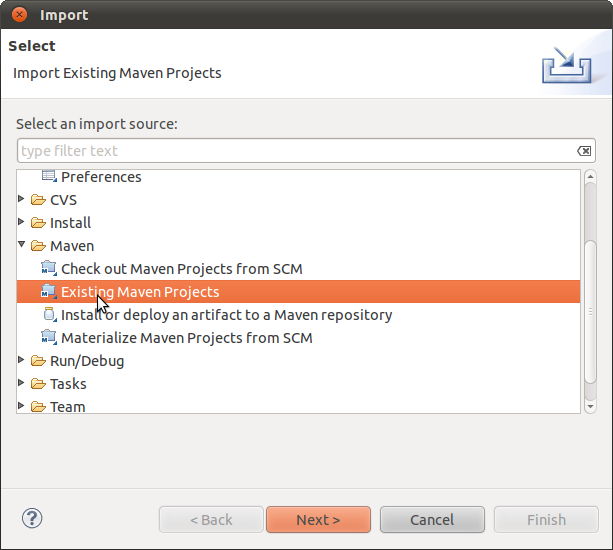
\includegraphics[width=\textwidth]{images/Screenshot-Import.png}

\item Click the \textbf{Browse} button
\item Select \textbf{cas} from \verb|/home/rice/workspace|

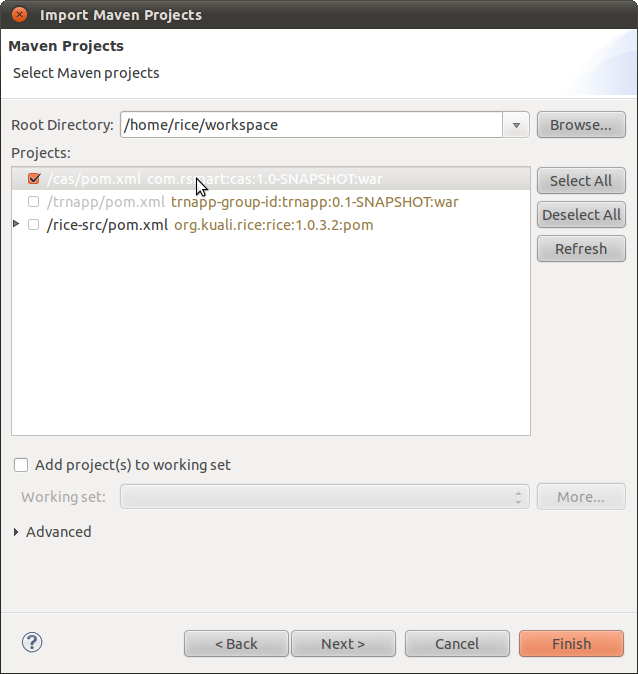
\includegraphics[width=\textwidth]{images/Screenshot14.png}
\item Edit \verb|src/main/resources/custom.properties|.

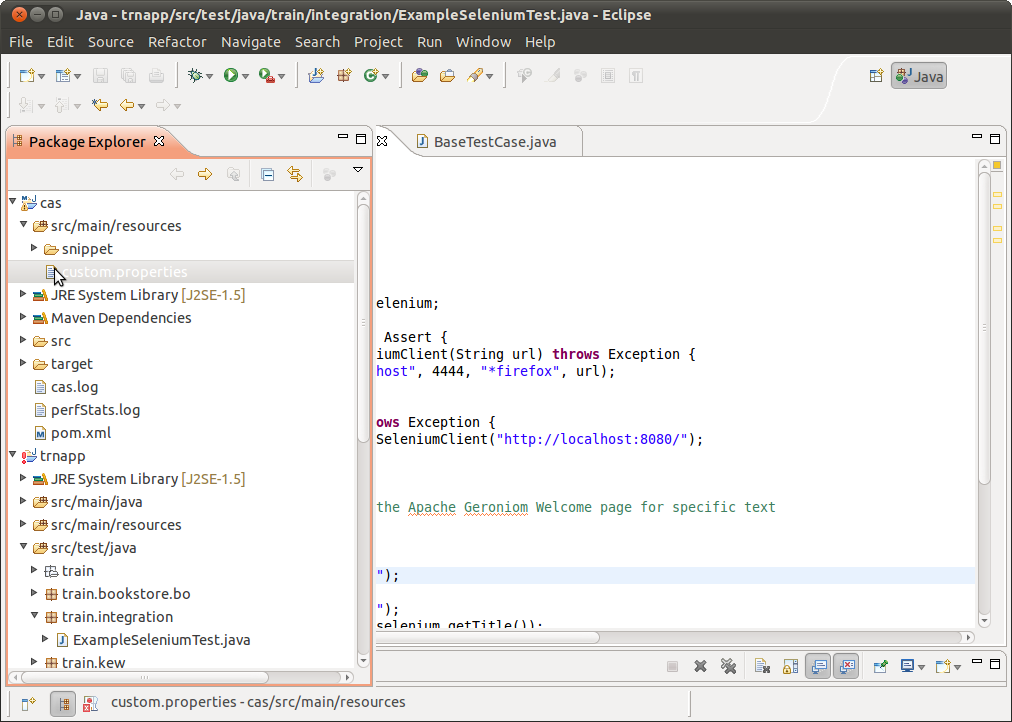
\includegraphics[width=\textwidth]{images/Screenshot15.png}
 You want it to look like this.
\begin{lstlisting}[language=bash,basicstyle=\scriptsize,backgroundcolor=\color{ubergray},caption={src/main/resources/custom.properties},frame=single,breaklines=true]
ldap.server.url=ldap://localhost
ldap.server.bind.username=cn=admin,dc=rsmart,dc=com
ldap.server.bind.password=rice
ldap.authentication.filter=eduPersonPrincipalName=%u,ou=people,dc=rsmart,dc=com
ldap.searchBase=ou=people,dc=rsmart,dc=com
\end{lstlisting}
\item Start it up with Maven
\begin{lstlisting}[language=bash,basicstyle=\scriptsize,backgroundcolor=\color{ubergray},caption={src/main/resources/custom.properties},frame=single,breaklines=true]
mvn war:inplace tomcat:run
\end{lstlisting}
\item Configure the application for CAS by editing the
  \verb|/home/rice/kuali/main/dev/trnapp-config.xml|
\begin{lstlisting}[numbers=left,language=xml,basicstyle=\scriptsize,backgroundcolor=\color{ubergray},caption={src/main/resources/custom.properties},frame=single,breaklines=true]
	<param name="rice.ldap.username">cn=admin,dc=rsmart,dc=com</param>
    <param name="rice.ldap.password">rice</param>
    <param name="rice.ldap.url">ldap://localhost</param>
    <param name="rice.ldap.base">ou=people,dc=rsmart,dc=com</param>
	<param name="rice.additionalSpringFiles">org/kuali/rice/kim/config/KIMLdapSpringBeans.xml</param>

      <param name="cas.rice.server.name">${application.host}:8081</param>
      <param name="cas.url">http://${cas.rice.server.name}/${cas.context.name}</param>
      <param name="cas.require.https">false</param>
      <param name="cas.validate.password">false</param>
       <param name="filter.login.class">org.jasig.cas.client.authentication.AuthenticationFilter</param>
       <param name="filter.login.casServerLoginUrl">${cas.url}/login</param>
       <param name="filter.login.serverName">${application.host}:${http.port}</param>
       <param name="filtermapping.login.1">/*</param>

       <param name="filter.validation.class">org.jasig.cas.client.validation.Cas20ProxyReceivingTicketValidationFilter</param>
       <param name="filter.validation.casServerUrlPrefix">${cas.url}</param>
       <param name="filter.validation.serverName">${application.host}:${http.port}</param>
       <param name="filtermapping.validation.2">/*</param>

       <param name="filter.caswrapper.class">org.jasig.cas.client.util.HttpServletRequestWrapperFilter</param>
       <param name="filtermapping.caswrapper.3">/*</param>
\end{lstlisting}
\item Browse to http://localhost:8081/cas/login

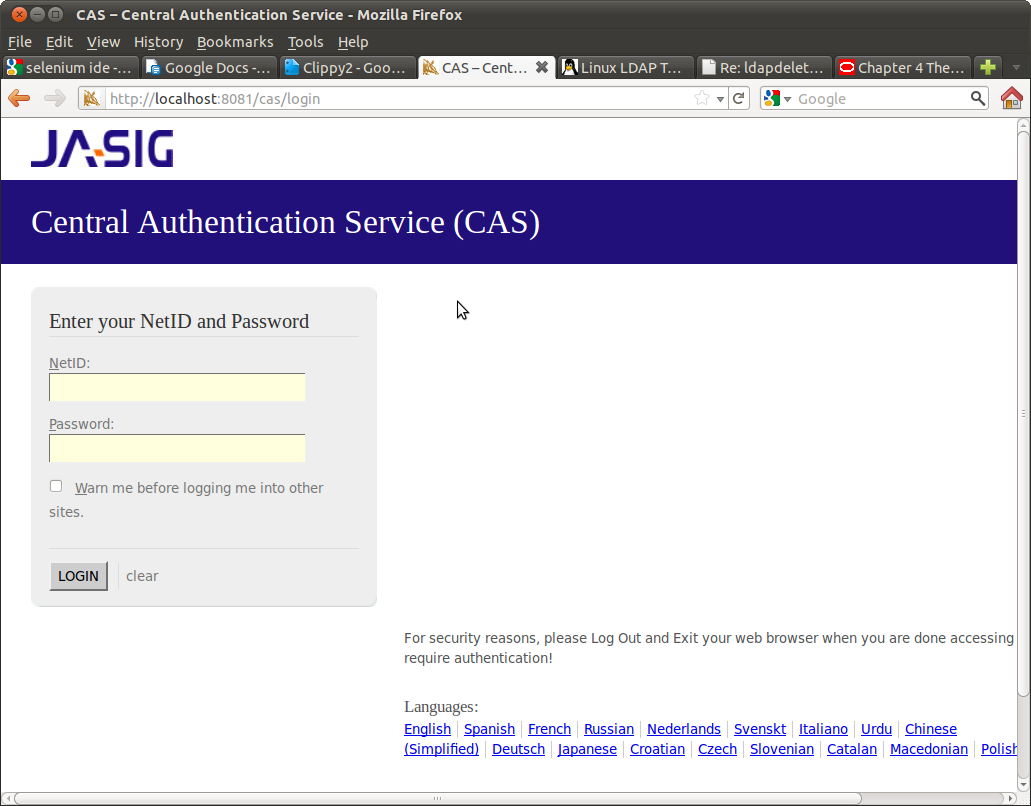
\includegraphics[width=\textwidth]{images/Screenshot16.png}

\end{enumerate}

\addcontentsline{toc}{subsection}{Add the Rice LDAP Integration Module}
\subsection*{2 Add the Rice LDAP Integration Module}
Add the LDAP Module to a Rice project and customize the mappers.

\addcontentsline{toc}{subsection}{Goals}
\subsection*{Goals}
\begin{enumerate}
  \item Learn to connect CAS to LDAP
  \item Learn to debug and troubleshoot LDAP Queries
  \item Learn to map between an LDAP database and KIM objects
  \item Learn to modify mappings at all levels
  \item Learn about caching in KIM
  \item Learn about configuring Rice LDAP Integration
\end{enumerate}

\addcontentsline{toc}{subsection}{Implementation}
\subsection*{1 Implementation}
\subsubsection*{1.1 Enable LDAP Integration}
\begin{enumerate}
\item Switch to the \verb|rice-src/ldap/| project
\item Browse to \verb|src/main/config/example-config/|
\item Open the rice-config.xml
\item Copy the contents into \verb|trnapp-config.xml|
\item Change the fields until they are like this:
\begin{lstlisting}[numbers=left,language=xml,basicstyle=\scriptsize,backgroundcolor=\color{ubergray},caption={trnapp-config.xml},frame=single,breaklines=true]
  <param name="rice.ldap.username">cn=admin,ou=people,dc=rsmart,dc=com</param>
  <param name="rice.ldap.password">rice</param>
  <param name="rice.ldap.url">ldap://localhost</param>
  <param name="rice.ldap.base">ou=People,dc=rsmart,dc=edu</param>
  <param
  name="rice.additionalSpringFiles">org/kuali/rice/kim/config/KIMLdapSpringBeans.xml</param>
\end{lstlisting}
This will turn the LDAP Integration on and configure the connection.
\end{enumerate}

\subsubsection*{1.2 Configure System Parameters}
\emph{These system parameters are so vital, that the application will fail
in most instances when not configured properly}
\begin{description}
\item [KIM\_TO\_LDAP\_FIELD\_MAPPINGS] Many different lookup for
  entities storied in LDAP can exist and they are not constrained to
  field name consistency. This means the field names can vary. In the
  event that field names do vary, then there cannot be a one-to-one
  mapping between KIM objects and LDAP objects. Instead, we have to
  have redundant mappings. This system parameter allows us to do just
  that.

When creating the System Parameters, use the following 

\begin{lstlisting}[language=sql,basicstyle=\scriptsize,backgroundcolor=\color{ubergray},caption={trnapp-config.xml},frame=single,breaklines=true]
entityId=uid;principalId=uid;principalName=eduPersonPrincipalName;givenName=sn;principals.principalName=eduPersonPrincipalName;persons.principalName=eduPersonPrincipalName;principals.principalId=uid;principals.active=employeeStatus;lastName=sn;firstName=givenName;employmentInformation.employeeStatus=employeeStatus;employmentInformation.employeeId=emplId,facultyId;names.lastName=sn;names.firstName=givenName;employmentInformation.employeeStatusCode=employeeStatus;
\end{lstlisting}

\item [KIM\_TO\_LDAP\_VALUE\_MAPPINGS] map possible values in the
  lookup form the results from an LDAP query. For example, employee
  active/inactive types have Y, N, and Both values. Each value needs
  to be mapped to a result from the LDAP query results.

\begin{lstlisting}[language=sql,basicstyle=\scriptsize,backgroundcolor=\color{ubergray},caption={trnapp-config.xml},frame=single,breaklines=true]
principals.active.Y=T;principals.active.N=!T;
\end{lstlisting}

\end{description}

\addcontentsline{toc}{subsection}{Use Case for Adding Caching}
\subsection*{2 Use Case for Adding Caching}

\newpage
{\setlength{\baselineskip}%
  {0.0\baselineskip}
  \section*{Notes}
  \hrulefill \par}